% !TeX program = xelatex
% 中国农业大学本科生毕业论文（设计）示例 — 文档结构编排
% 编译：latexmk -xelatex main.tex
% --------------------------------------------------------------
% 写作分工：
%   - 个人信息 / 占位变量 → info.tex
%   - 各章节内容          → sections/*.tex
%   - 参考文献条目        → refs/refs.bib
%   - 本文件只负责加载和组织
% --------------------------------------------------------------
\documentclass{cauugthesis}

\usepackage{tikz}
\usetikzlibrary{arrows.meta,positioning}

\graphicspath{{../../logo/}{figures/}}
\setcounter{tocdepth}{2}
\setcounter{secnumdepth}{3}

% ============================================================
% info.tex — 本科生毕业论文（设计）基本信息（SSOT）
% ============================================================
% 全篇所有需要个人填写的字段都集中在这一个文件。改一处，封面、
% 页眉、致谢所有相关位置自动同步。其余章节文件 (sections/*.tex)
% 只写论文内容，不需要再放姓名、日期等元数据。
%
% 编辑顺序建议：
%   ① 第 1 区：填封面字段
%   ② 第 2 区：注册正文反复出现的占位串（研究对象、数据集名、方法名…）
% ============================================================

% ---------- 1. 封面字段 ----------
\thesistitle{【中文论文题目：请替换为最终题目】}
\thesistitleen{【English Thesis Title: Replace with the Final Title】}
\thesisauthor{【学生姓名】}
\advisor{【导师姓名】\quad 【职称】}
\coadvisor{}                                                % 合作指导教师，无则留空
\major{【专业名称】}
\college{【学院名称】}
\thesisdate{【20XX 年 X 月】}

% ---------- 2. 正文可复用变量 ----------
% 在正文里用 \thevar{key} 引用；改这里全文统一。
% 未注册的 key 编译时给警告，便于排查。
\thesisvar{研究对象}{【研究对象，如：冬小麦】}
\thesisvar{数据集}{【数据集名称，如：Sentinel-2 时序】}
\thesisvar{方法名}{【本文方法的简称】}
\thesisvar{研究区}{【研究区或实验平台】}
                            % 所有个人信息和复用变量都在这里

\begin{document}

% ---------- 前置部分 ----------
\makecover
\makedeclaration
\frontmatterpages

\begin{cnabstract}{【关键词一】；【关键词二】；【关键词三】；【关键词四】}
【第一段：研究背景与问题。说明研究对象、应用场景和当前瓶颈。建议用 250--350 字交代为什么这个问题值得研究，避免在摘要中展开文献综述。】

【第二段：数据与方法。说明研究区、数据来源、样本构建、核心模型或实验设计。可以按“本文以……为对象，构建……数据集，采用……方法，实现……”组织。】

【第三段：主要结果。给出可核验的定量结果，如精度指标、对比提升、关键参数或显著性结论。没有最终数值时先用“【R2=】”“【RMSE=】”等占位，定稿前必须替换。】

【第四段：结论与意义。概括方法贡献、适用范围和局限。摘要中不要引入正文没有支撑的新判断。】
\end{cnabstract}

\begin{enabstract}{【keyword one】; 【keyword two】; 【keyword three】; 【keyword four】}
【Paragraph 1: Background and research gap. State the object, application scenario, and the limitation addressed by the thesis.】

【Paragraph 2: Data and methods. Describe the study area, datasets, feature construction, model, and validation protocol.】

【Paragraph 3: Main results. Report quantitative metrics and the most important empirical findings with placeholders replaced before submission.】

【Paragraph 4: Conclusion and implications. Summarize the contribution, scope of application, and remaining limitations.】
\end{enabstract}

\maketoc
\makefigurelist

\begin{symbollist}
  【符号】 & 【含义】 & 【单位】 \\
  $x_i$ & 第 $i$ 个样本的输入特征 & -- \\
  $y_i$ & 第 $i$ 个样本的观测值 & 【单位】 \\
  $\hat{y}_i$ & 第 $i$ 个样本的预测值 & 【单位】 \\
\end{symbollist}

% ---------- 正文 ----------
\startmainbody

\section{绪论}\label{ch:intro}

\subsection{研究背景与意义}

【本节填写研究问题的现实背景。建议从应用场景写起：研究对象是什么，为什么重要，当前实践或已有方法遇到了什么限制。】

以农业、生态、工程或信息类论文为例，背景段可以采用“对象--需求--瓶颈--本文切入点”的顺序组织。第一段说明研究对象及其应用价值；第二段说明已有技术路线；第三段指出仍未解决的问题，并自然引出本文工作。

\subsection{国内外研究现状}

【本节填写文献综述。建议按方法类别或问题链条分小节，不要按论文逐篇罗列。每个段落以判断句开头，再用文献支撑。】

已有研究通常可以分为经验统计方法、机理模型方法和数据驱动方法三类。经验统计方法实现简单，但跨场景迁移能力有限；机理模型解释性较强，但参数反演存在不确定性；数据驱动方法能够刻画复杂非线性关系，但对训练样本和评估设计较为敏感\citep{breiman2001random,verrelst2015optical}。

\subsubsection{经验统计方法}

【三级标题示例。用于展开二级标题下的具体方向、实验步骤或子问题。三级标题会在正文中编号为 1.2.1，但目录默认只列到二级标题。】

经验统计方法通常以少量可解释变量建立目标变量的回归关系，优点是实现简单、结果直观，缺点是模型参数容易受研究区、样本范围和观测条件影响。

\subsubsection{数据驱动方法}

【三级标题示例。若某一二级标题下存在多个并列方法或实验环节，建议使用三级标题，而不是用加粗段首替代正式层级。】

数据驱动方法能够从高维特征中学习复杂非线性关系，但需要关注样本代表性、数据泄露、过拟合和跨场景验证等问题。

\subsection{研究内容与技术路线}

【本节填写本文具体做什么。建议列出 3--4 项工作，每项都能在后文章节找到对应实验或结果。】

本文围绕【研究对象】开展如下工作：

（1）构建【数据集或实验样本】，完成【预处理、配准、质量控制】等步骤；

（2）设计【模型或方法】，提取【关键特征】，建立【输入--输出】映射关系；

（3）通过【交叉验证/消融实验/对比实验】评估模型性能，分析主要误差来源；

（4）总结方法适用范围，并提出后续改进方向。

\begin{figure}[ht]
  \centering
  \begin{tikzpicture}[
    node distance=6mm,
    box/.style={draw, rounded corners=2pt, minimum width=29mm, minimum height=9mm, align=center},
    arrow/.style={-{Latex[length=2.5mm]}, thick}
  ]
    \node[box] (data) {数据获取\\与预处理};
    \node[box, right=of data] (feature) {特征构建\\与样本筛选};
    \node[box, right=of feature] (model) {模型训练\\与验证};
    \node[box, right=of model] (analysis) {结果分析\\与应用评价};
    \draw[arrow] (data) -- (feature);
    \draw[arrow] (feature) -- (model);
    \draw[arrow] (model) -- (analysis);
  \end{tikzpicture}
  \caption{本文技术路线示意图}
  \label{fig:workflow}
\end{figure}

\subsection{论文组织结构}

本文共分为五章。第一章介绍研究背景、研究现状和技术路线；第二章说明研究区、数据来源和预处理流程；第三章介绍核心方法与评价指标；第四章展示实验结果并开展讨论；第五章总结主要结论、创新点和不足。

\section{材料与数据}\label{ch:data}

\subsection{研究区概况}

【填写研究区位置、自然条件、实验对象和数据采集背景。若论文不是地理或农业方向，可将本节改为“实验对象与样本来源”。】

研究区位于【省/市/县或实验平台名称】，地理范围为【经纬度或空间范围】。研究对象为【作物/材料/系统/设备】，数据采集时间为【日期范围】。研究区或实验对象的基本情况见表\ref{tab:study-area}。

\begin{table}[ht]
  \centering
  \caption{研究区或实验对象基本信息}
  \label{tab:study-area}
  \begin{tabular}{lll}
    \toprule
    项目 & 内容 & 说明 \\
    \midrule
    研究对象 & 【填写】 & 【如作物类型、样本类型】 \\
    时间范围 & 【填写】 & 【如 20XX 年 X 月至 X 月】 \\
    数据规模 & 【填写】 & 【如样本数、影像数、观测次数】 \\
    空间尺度 & 【填写】 & 【如像元、样方、实验单元】 \\
    \bottomrule
  \end{tabular}
\end{table}

\subsection{数据来源}

【填写原始数据来源、仪器设备、公开数据集或人工标注流程。需要说明数据格式、分辨率、采样频率、坐标系统或实验条件。】

本文使用的数据包括【数据 A】、【数据 B】和【辅助数据】。其中，【数据 A】用于表征【输入信息】，【数据 B】用于提供【标签或验证信息】，【辅助数据】用于【质量控制或空间配准】。

\begin{longtable}{lll}
\caption{主要数据源及用途}\label{tab:data-source}\\
\toprule
数据类型 & 主要内容 & 用途 \\
\midrule
\endfirsthead
\toprule
数据类型 & 主要内容 & 用途 \\
\midrule
\endhead
\bottomrule
\endfoot
【数据 A】 & 【分辨率/字段/格式】 & 【特征提取】 \\
【数据 B】 & 【分辨率/字段/格式】 & 【标签构建或验证】 \\
【辅助数据】 & 【分辨率/字段/格式】 & 【筛选、配准或解释】 \\
\end{longtable}

\subsection{数据预处理}

【填写预处理流程。建议按实际执行顺序写：格式转换、异常值剔除、坐标统一、空间/时间匹配、归一化、样本筛选。】

预处理包括以下步骤：首先，对原始数据进行格式统一和异常值检查；其次，将不同来源数据配准到统一坐标或样本索引；最后，根据质量控制规则剔除无效样本，形成可用于建模的样本表。

设原始观测值为 $x$，归一化后的特征为 $x'$，本文采用的 min--max 归一化公式为
\begin{equation}
x' = \frac{x - x_{\min}}{x_{\max} - x_{\min}}.
\end{equation}

其中，$x_{\min}$ 和 $x_{\max}$ 分别表示训练集中该特征的最小值和最大值。验证集和测试集仅使用训练集统计量进行变换，以避免数据泄露。

\section{研究方法}\label{ch:method}

\subsection{总体框架}

【本节填写方法流程。建议先给总体框架，再分别介绍特征、模型、训练和评价。】

本文方法由四部分组成：样本构建、特征提取、模型训练和精度评价。给定样本集合 $\{(x_i,y_i)\}_{i=1}^{n}$，其中 $x_i$ 为输入特征，$y_i$ 为目标变量，模型学习映射函数 $f(\cdot)$，并输出预测值 $\hat{y}_i=f(x_i)$。

\subsection{特征构建}

【填写输入特征。若使用遥感影像，可写波段、指数、纹理、结构特征；若使用表格数据，可写统计量、类别变量编码和衍生变量。】

特征构建遵循“物理含义明确、尺度一致、避免冗余”的原则。表\ref{tab:feature-groups}列出了示例特征组，实际使用时应替换为论文真实特征。

\begin{table}[ht]
  \centering
  \caption{特征组示例}
  \label{tab:feature-groups}
  \begin{tabular}{lll}
    \toprule
    特征组 & 示例变量 & 含义 \\
    \midrule
    原始观测 & 【变量 1--变量 k】 & 【直接观测信息】 \\
    统计特征 & 均值、标准差、分位数 & 【局部或时间窗口统计】 \\
    指数特征 & 【指数 A】、【指数 B】 & 【组合变量或机理指标】 \\
    辅助特征 & 【地形/时间/类别】 & 【解释异质性】 \\
    \bottomrule
  \end{tabular}
\end{table}

\subsection{模型构建}

【填写模型名称、输入输出、关键参数和训练策略。不要只写软件包名称，要说明为什么该模型适合本问题。】

\subsubsection{模型输入与输出}

【三级标题示例。这里可说明输入张量、特征表、图像块或序列数据的形状，以及模型输出的变量含义。】

设模型输入为 $x_i$，输出为 $\hat{y}_i$。若输入包含多源数据，应分别说明各数据源的维度、单位、时间或空间对齐方式。

\subsubsection{训练策略}

【三级标题示例。这里可说明训练集、验证集、测试集划分，损失函数、优化器、学习率、随机种子和早停策略。】

本文采用【模型名称】建立输入特征与目标变量之间的非线性关系。模型训练以均方误差为基础损失函数：
\begin{equation}
\mathcal{L}_{\mathrm{MSE}} = \frac{1}{n}\sum_{i=1}^{n}(y_i-\hat{y}_i)^2.
\end{equation}

为提升结果稳定性，训练过程采用【交叉验证/重复实验/独立测试集】。所有超参数仅在训练集和验证集上确定，测试集仅用于最终性能报告。

\subsection{评价指标}

【填写评价指标。回归问题常用 R2、RMSE、MAE；分类问题可替换为 Accuracy、F1、AUC 等。】

本文采用决定系数 $R^2$、均方根误差（RMSE）和平均绝对误差（MAE）评价模型精度：
\begin{equation}
R^2 = 1 - \frac{\sum_{i=1}^{n}(y_i-\hat{y}_i)^2}{\sum_{i=1}^{n}(y_i-\bar{y})^2},
\end{equation}
\begin{equation}
\mathrm{RMSE} = \sqrt{\frac{1}{n}\sum_{i=1}^{n}(y_i-\hat{y}_i)^2},
\end{equation}
\begin{equation}
\mathrm{MAE} = \frac{1}{n}\sum_{i=1}^{n}|y_i-\hat{y}_i|.
\end{equation}

其中，$\bar{y}$ 为观测值均值。$R^2$ 越接近 1 表明模型解释能力越强，RMSE 和 MAE 越小表明预测误差越低。

\section{结果与分析}\label{ch:results}

\subsection{数据统计特征}

【本节填写数据分布和质量检查结果。建议先描述样本量、均值、范围和异常值，再解释这些统计特征对建模的影响。】

样本统计结果见表\ref{tab:sample-stat}。从示例结果可以看出，不同数据子集在样本量和目标变量均值上存在差异，因此后续建模需要关注数据划分是否引入偏差。

\begin{table}[ht]
  \centering
  \caption{样本统计信息示例}
  \label{tab:sample-stat}
  \begin{tabular}{lrrrr}
    \toprule
    数据子集 & 样本量 & 均值 & 标准差 & 范围 \\
    \midrule
    训练集 & 【填写】 & 【填写】 & 【填写】 & 【填写】 \\
    验证集 & 【填写】 & 【填写】 & 【填写】 & 【填写】 \\
    测试集 & 【填写】 & 【填写】 & 【填写】 & 【填写】 \\
    \bottomrule
  \end{tabular}
  \tablenote{表中数值为占位示例，定稿前应替换为真实统计结果。}
\end{table}

\subsection{模型精度评价}

【本节填写核心结果。建议所有主要结论都绑定表格或图，避免只给定性描述。】

图\ref{fig:result-map}展示了模型预测结果的空间分布。可以看出，预测值在【高值区域】和【低值区域】之间存在明显差异，说明模型能够刻画研究对象的空间异质性。

\begin{figure}[ht]
  \centering
  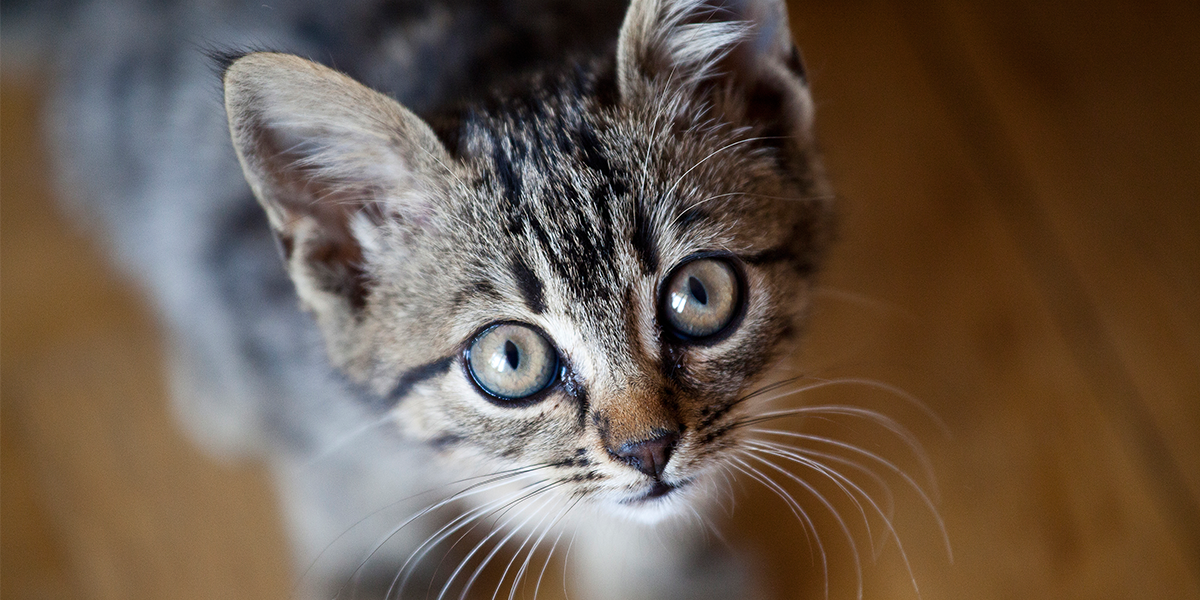
\includegraphics[width=0.78\textwidth]{fig1.png}
  \caption{模型预测结果空间分布示例}
  \label{fig:result-map}
  \figurenote{底图为示例图片，定稿时应替换为论文真实结果图，并在图注中说明颜色、符号或分组含义。}
\end{figure}

不同模型或不同实验方案的精度对比如表\ref{tab:model-performance}所示。结果表明，【模型 A】在测试集上取得最优表现，说明【解释原因】。

\begin{table}[ht]
  \centering
  \caption{模型性能对比示例}
  \label{tab:model-performance}
  \begin{tabular}{lrrr}
    \toprule
    方法 & $R^2$ & RMSE & MAE \\
    \midrule
    基准模型 & 【填写】 & 【填写】 & 【填写】 \\
    对比模型 & 【填写】 & 【填写】 & 【填写】 \\
    本文方法 & 【填写】 & 【填写】 & 【填写】 \\
    \bottomrule
  \end{tabular}
  \tablenote{$R^2$ 越大表示拟合效果越好，RMSE 和 MAE 越小表示预测误差越低。}
\end{table}

\subsection{消融实验}

【若论文包含模型改进，建议增加消融实验。每次只移除或替换一个组件，说明该组件是否真的有效。】

消融实验结果见表\ref{tab:ablation}。与完整方案相比，移除【组件 A】后精度下降，说明该组件对模型性能具有贡献。

\begin{table}[ht]
  \centering
  \caption{消融实验结果示例}
  \label{tab:ablation}
  \begin{tabular}{lrrr}
    \toprule
    实验方案 & $R^2$ & RMSE & 相对变化 \\
    \midrule
    完整方案 & 【填写】 & 【填写】 & -- \\
    去除组件 A & 【填写】 & 【填写】 & 【填写】 \\
    去除组件 B & 【填写】 & 【填写】 & 【填写】 \\
    \bottomrule
  \end{tabular}
\end{table}

\subsection{讨论}

【讨论不是重复结果，而是解释结果为什么发生、与已有研究是否一致、限制在哪里。建议按“现象--原因--证据--影响”组织。】

本文结果与已有研究中关于【现象】的结论基本一致\citep{meyer2021predicting}。可能原因在于【机制解释】。同时，本文仍存在【数据覆盖/模型假设/验证设计】方面的限制，后续需要通过更多样本或更严格的独立验证进一步检验。

\section{结论与展望}\label{ch:conclusion}

\subsection{主要结论}

【结论应直接回应研究内容，不要写成摘要的缩写。建议 3--4 条，每条包含“做了什么”和“得到什么结果”。】

（1）本文构建了【数据集/实验流程】，完成了【关键处理步骤】，为【研究问题】提供了可复现的数据基础。

（2）本文提出或采用了【方法名称】，通过【特征/模型/实验设计】实现了【目标任务】，在【测试集/验证集】上取得【指标】。

（3）对比实验和消融实验表明，【关键组件或变量】对性能提升具有主要贡献，说明【机制或应用意义】。

\subsection{创新点}

【本科论文的创新点可以是数据、方法、流程或应用层面的局部创新。避免夸大为“首次”“国际领先”，除非有充分证据。】

（1）数据层面：【填写数据组织、标注、配准或质量控制上的改进】。

（2）方法层面：【填写模型、特征、实验设计或评价方式上的改进】。

（3）应用层面：【填写该方法对实际问题的支撑价值】。

\subsection{不足与展望}

【本节应具体，不要只写“样本量较少、模型有待提高”。建议说明不足如何影响结论，以及下一步怎么解决。】

本文仍存在以下不足：首先，【数据覆盖范围】有限，可能影响模型在其他场景下的泛化能力；其次，【模型或假设】仍较简化，尚未充分考虑【因素】；最后，【验证方式】仍需在独立数据上进一步检验。

后续研究可从三个方面推进：第一，扩充【时间/空间/对象】维度的数据集；第二，引入【更强模型或机理约束】提升解释性与稳定性；第三，面向实际应用构建自动化处理流程，提高方法可复现性和部署效率。


% ---------- 后置部分 ----------
\bibliography{refs/refs}

\begin{acknowledgements}
【致谢正文。建议感谢导师、课题组、数据或实验支持人员、同学朋友和家人。避免使用夸张措辞，保持真实、具体、简洁。】

\begin{flushright}
  \textit{\thethesisauthor} \\
  \thethesisdate
\end{flushright}
\end{acknowledgements}

\begin{appendixsection}{补充材料}
【附录用于放置正文中过长但仍有参考价值的内容，例如补充表格、参数列表、问卷、代码片段或额外图件。】

\begin{table}[ht]
  \centering
  \caption{主要参数设置示例}
  \begin{tabular}{lll}
    \toprule
    参数 & 取值 & 说明 \\
    \midrule
    【参数 A】 & 【填写】 & 【填写】 \\
    【参数 B】 & 【填写】 & 【填写】 \\
    【参数 C】 & 【填写】 & 【填写】 \\
    \bottomrule
  \end{tabular}
\end{table}

\end{appendixsection}

\begin{authorinfo}
\textbf{基本介绍：}【姓名】，性别【填写】，出生于【YYYY 年 MM 月 DD 日】，籍贯【填写】。

\textbf{教育经历：}【高中/本科等教育经历，按时间顺序填写】。

\textbf{本科期间发表的学术论文：}【无 / 论文题目、期刊或会议、作者顺序】。

\textbf{本科期间主持/参与的科研项目：}【无 / 项目名称、项目来源、本人职责】。

\textbf{本科期间获得的奖励和荣誉：}【无 / 奖项名称、等级、时间】。

\textbf{其他成果：}【无 / 软件著作权、竞赛、专利、开放数据或其他成果】。

\end{authorinfo}

\end{document}
